\documentclass{article}

\usepackage[pdfstartview=FitH,colorlinks=false,urlcolor=blue]{hyperref}
\usepackage{graphicx}
\usepackage{fullpage}
%\setcounter{secnumdepth}{0}
\begin{document}

\graphicspath{{images/}}
\title{A Log Structured File System with Snapshots}
\author{Pradeep Padala \\
EECS, University of Michigan\\
e-mail: ppadala@umich.edu}%

\maketitle

\section{Introduction}

A log structured file system (LFS) \cite{Rosenblum91} writes all the file
system data sequentially in a \textit{log-like} structure. A log consists of a
series of \textit{segments} where each segment contains both data and inode
blocks.  Traditional file systems like \texttt{ext2} usually write inode
blocks at a fixed place on the disk, causing overhead due to disk seeks. A log
structured file system gathers a segment worth of data in memory and appends
the segment at the end of the log.  This dramatically improves the write
performance while maintaining the same read performance. The sequential
nature of the log also helps in crash recovery as less checkpointing
information need to be stored.  As the file system grows and files are
deleted, holes are created in the file system. A \textit{cleaner} is required
to fill the holes and compact the file system allowing large extents of free
blocks to be found. The novel aspect in our work is the addition of
snapshotting capability to log-structured file systems. Currently, no Linux
file system offers this capability.

The primary objective of this work is to create a log-structured file system
for Linux that supports snapshots. A snapshot is a copy of the files taken at
a particular time. This is very similar to backup of a file system at a
particular time except that it is maintained within the same file system
without wasting any space. We
believe that LFS is the ideal file system for maintaining snapshots, because
its design renders naturally to maintain snapshots.

\section{Motivation}
\textit{Why do we need yet another file system for Linux?} When LFS was
originally proposed, the idea of \textit{append-to-end-of-log} to improve
write performance was novel and produced great results on various micro
benchmarks. However, later studies \cite{log_vs_cluster} have shown that in
transaction processing environments LFS performs poorly due to the cleaner
overhead.  We believe that advances in disk and memory technologies will help
log structured file systems. In the past decade, huge improvements are seen in
the disk and memory sizes for a typical machine. Increase in memory size
allows LFS to gather more segments in memory and with larger disk space, the
cleaner need not be run as often.

Currently, no Linux file system supports snapshots. Snapshots are usually
considered a special capability supported by network attached storage devices
(NASD) developed by companies like NetApp. The cost of these NASDs is
prohibitive for small businesses and we believe that we can develop an open
source file system that supports snapshots. Since LFS lends itself naturally
to support snapshots, we propose to implement an LFS for Linux.

\section{Deliverables}
\begin{itemize}
\item
\textbf{LFS kernel module}:
A file system module implementing the core functionality of LFS that provides basic
file system capabilities. The kernel module will work with the latest stable
kernel ($>=$ \texttt{2.6.0}).
\item
\textbf{mkfs.lfs}:
A program for creating LFS partitions.
\item
\textbf{dbg.lfs}:
A program that provides access to on-disk LFS data structures without the
kernel module.
\item
\textbf{clean.lfs}:
A program for regenerating empty segments by cleaning heavily fragmented
segments.
\item
\textbf{Documentation}:
Basic documentation describing the capabilities of LFS and how it should be
used. The code will contain the necessary comments to understand and extend
it.
\item
\textbf{Basic snapshotting capability}:
We hope to complete basic snapshotting capability supporting two versions of
files by the end of the SoC program. We hope to improve it to multiple
versions in future.
\end{itemize}

\section{Project details}
In the next few sections, we describe the basic operations in LFS and how
they differ from traditional file systems. We also provide details of
cleaning, snapshotting algorithms and preliminary data structures we have 
designed for LFS.

\subsection{General layout}

General layout of an LFS is shown in Figure \ref{gen_struct}. An LFS consists
of a super block and a series of segments. Each segment contains a segment
summary identifying the blocks in the segment.  The segment may contain both
data and inode blocks. Section \ref{ds} contains more details about the
segment summary data structure.

\subsection{Reading a file}
\begin{figure}
\centering
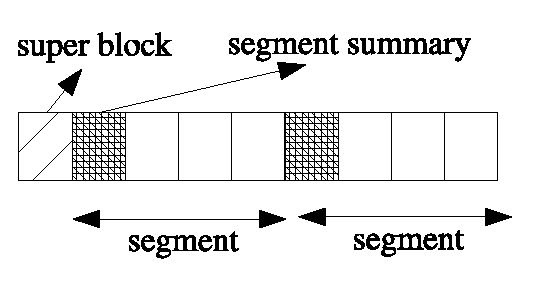
\includegraphics[scale=0.7]{lfs1}
\caption{General layout of an LFS}
\label{gen_struct}
\end{figure}

To enable random access retrieval from the LFS, the log contains indexing
information. The basic structures used to enable this random  access retrieval 
are similar to those used in traditional UNIX file systems.

Each file is assigned an inode, which contains information of the disk
addresses of the first ten blocks of the file; for larger files it would
contain address of one or more data or indirect blocks. Besides disk
addresses, an inode would also contain file parameters like access permissions
and modify times. In a traditional Unix file system, the inodes are at a fixed
place, whereas in LFS, inodes are written to the log and an inode map is used
to maintain the current location of a particular inode. Given the identifying
number for a file, the inode map is indexed to give the disk address for the
inode of that file. The inode map is also written to the log as a file (called
IFILE). Note that this is different from the traditional file systems, where
inode map is stored at a fixed region. The block address for IFILE inode is
stored in the superblock.

\subsection{Creating and Writing files}
\begin{figure}
\centering
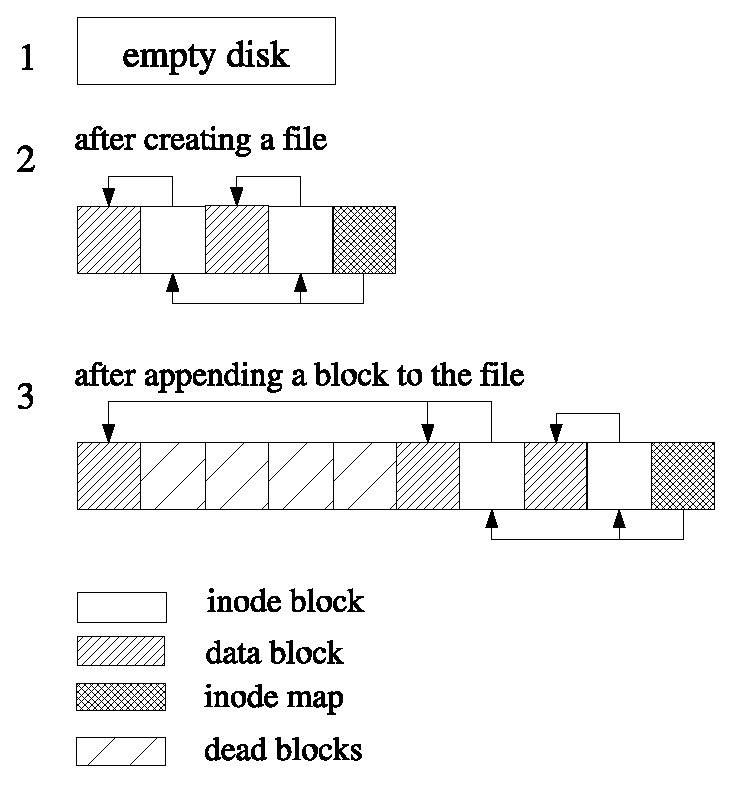
\includegraphics[scale=0.7]{lfs2}
\caption{Creating and writing to a file}
\label{create}
\end{figure}


In an LFS, new blocks are always written to the end of the log. We show an
example of file creation to highlight the differences between a traditional
file system and LFS. Figure \ref{create} shows the creation of a file and
appending a block to the file. Initially we have an empty disk as shown in
(1). When a file is created, its data block and inode block are written to the
end of the log.  Then, the directory containing the file is updated
appropriately by writing the directory data and inode blocks. Finally, the
IFILE blocks are written to the log. (3) shows the appending a
block to the file. New blocks are written to the end of the log and the
metadata pointers are updated accordingly as shown in the figure.

Note that the blocks are not written individually, but are written only
after gathering a segment worth of blocks in memory.

\subsection{Cleaning}
\begin{figure}
\centering
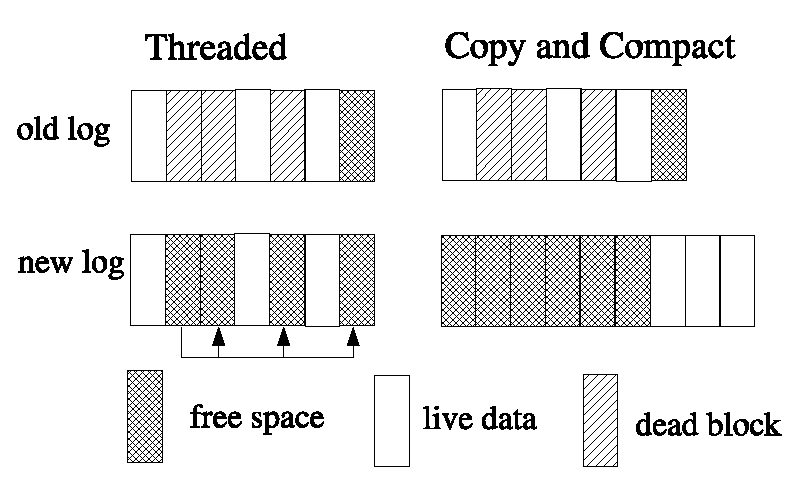
\includegraphics[scale=0.7]{lfs3}
\caption{Cleaning mechanisms}
\label{cleaning}
\end{figure}


One of the key aspects in a log structured file system is to maintain large extents of
disk blocks for writing new segments. As more and more updates are done to the
file system, holes (dead data) are created in the file system. A program
called cleaner is required to reclaim these holes and compact the live data.
There are two ways for maintaining the log with holes: threading and copying.
In a threaded log, live data is left in place and special data
structures are used to thread the log through free extents. This approach
becomes quickly infeasible because of the fragmentation caused by updates. The
second approach is to compact the live data to create large free extents.
These approaches are shown in Figure \ref{cleaning}.

In this project, we will be using a combination of threading and copying. In
this approach, we create free segments by copying the live data to new segments
and threading to identify the free segments. The live data is always
written to the end of the log. However, the log is threaded to identify the
free segments quickly.

\subsubsection{Cleaning Algorithm}
Segment compaction is a three-step process as outlined below.
\begin{enumerate}
\item
Read certain number of segments into memory.
\item
Identify live data by using the information in the segment summary.
\item
Prepare new segments containing only the live data and write these to the end
of the log.
\item
Mark the old segments free. These segments can be used for future writes.
\end{enumerate}

The key aspect of the cleaning algorithm is the segments that are used for
copying. We want to quickly identify the segments with the most dead data.
The \textit{segment summary} data structure is used to identify segments that
can be cleaned. This data structure is updated as changes are made to the file
system.

\subsubsection{Cleaning policies}
The following policy issues need to be addressed for cleaning.
\begin{itemize}
\item
When should the cleaner execute? The cleaner could be run continuously along
with normal file system activity or run it at a time when the system load is
minimal. Since we will be supporting snapshots, the amount of data that needs
to be claimed is minimal. Running the cleaner at night should be sufficient
for a typical machine.
\item
How many segments should be cleaned? We use the \textit{write cost} as
explained in \cite{Rosenblum91} to decide the number of segments to be
cleaned. The statistics required for measuring this cost are maintained in the
segment usage table.
\item
Which segments should be cleaned? Ideally, we would like to clean the segments
with the most dead blocks. We will use a threshold to identify a list of
segments that can be cleaned along with the \textit{write cost} as explained in
\cite{Rosenblum91}.
\item
How should the live blocks be grouped? A good heuristic is to group blocks of
similar age into new segments. Another heuristic is to group blocks of related
files (for example, all the files in a directory).
\end{itemize}

\subsection{Snapshots}

\begin{figure}
\centering
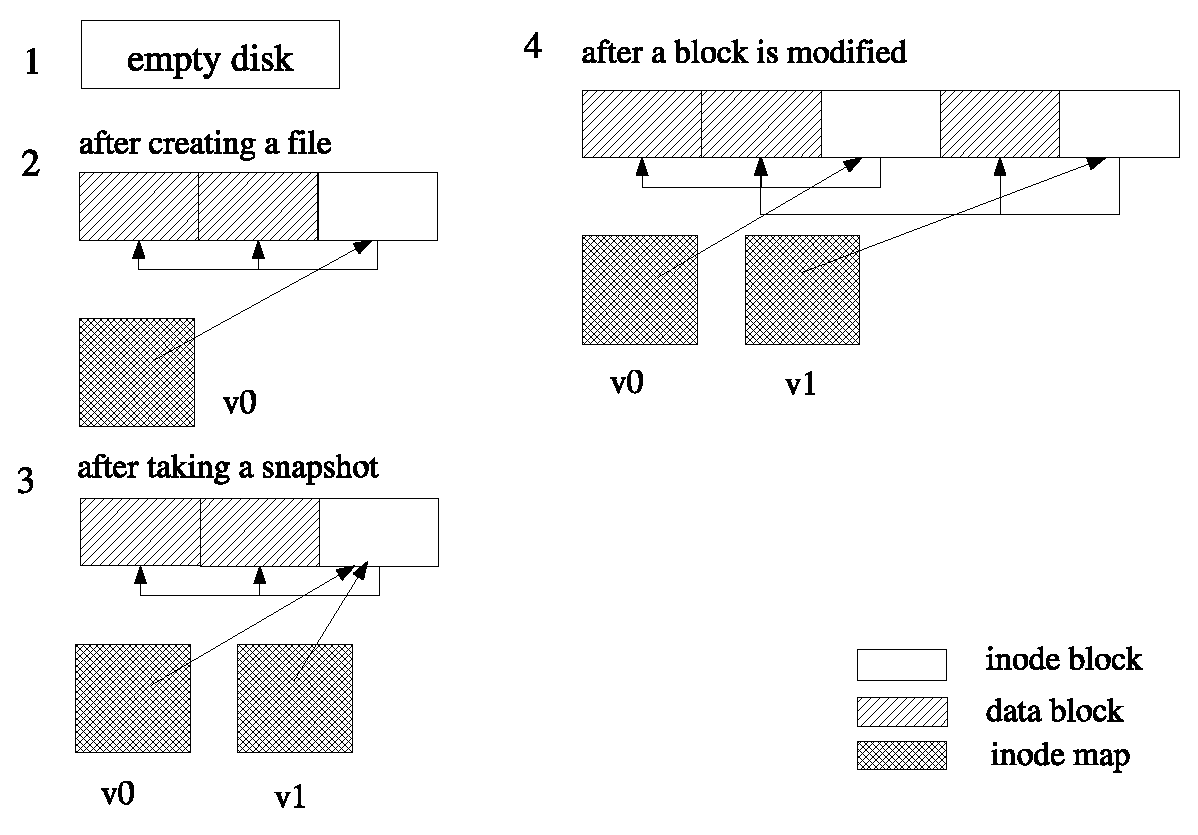
\includegraphics[scale=0.6]{lfs4}
\caption{Snapshots}
\label{snap}
\end{figure}


The novel aspect in our work is the snapshotting capability for log-structured
file systems. One of the first file
systems to introduce snapshotting is Write Anywhere File Layout (WAFL) file
system \cite{wafl} that adds snapshotting on top of an existing ext2 like file
system. 

Here, we describe the mechanism for maintaining snapshots in an LFS. In Figure
\ref{snap} (1) shows the empty disk and (2) shows the file system after a file
containing two data blocks is created. For clarity, directory inodes are
omitted. These blocks belong to the first version of the file and the inode
map points to the file inode. After a snapshot is taken, a new inode map is
created that is an exact replica of the old version as shown in (3). As soon as a modification
is done, the new inode map will point to the new set of blocks as shown in
(4). Note that the inode map itself is a file in our file system and
modification of inode map results in new inode blocks being written to the
disk.

Since this mechanism lends very nicely with the \textit{append-to-end-of-log}
property, log-structured file systems are well suited for maintaining
snapshots.

The key question is \textit{how do we handle cleaning with snapshots?}
Note that when we want to
remove a snapshot, we cannot simply clean all the inodes and data blocks in
that snapshot. There might be inodes from other snapshots pointing to the
block we are trying to clean.

The original LFS \cite{Rosenblum91} used the version number to quickly identify whether a
block can be reclaimed or not. Unfortunately, this mechanism no longer works
with snapshots. We propose the addition of a snapshot map for finding out
whether a block can be cleaned or not. The snapshot map contains a reference
count for all the blocks in the file system. A reference count zero means
there are no snapshots pointing to the data block. The snapshot can be
maintained at a fixed location on the disk or can be written to the log
similar to the IFILE.

\subsection{Performance Evaluation}
We will perform a basic evaluation of LFS comparing it to modern file
systems like ext3 and reiserfs. We will compare the performance of basic
low level operations like read and write and high level operations similar to
the operations described in \cite{fs_bench}.

For future work, we want to measure the performance of LFS in certain
scenarios where file writes are dominated by appends. Google reported this
behavior in their workloads while describing their distributed file system
GFS \cite{googlefs}. Log-structured file systems are tailor-made for 
\textit{append-only} scenarios.

\subsection{Preliminary data structures}
\label{ds}
We provide brief details of the required data structures and what they should
contain. The structures are designed after considering the earlier BSD LFS
and current Linux file system implementations. These are described 
in pseudo C syntax. Note that more fields will be added to these structures in
future.
\begin{itemize}
\item
\textbf{Superblock}: In traditional file systems, superblock contains the
necessary information to mount a file system. Along with the usual fields,
superblock for LFS should have the following fields.
\begin{verbatim}
struct lfs_super_block {
    u32 s_ifile_iaddr;  /* IFILE inode block number */
    u32 s_nino;	        /* Number of allocated inodes in the system */
    u32 s_next_seg;     /* Block number of the next segment */
    u32 s_segsize;      /* Segment size in our file system  in blocks */
};
\end{verbatim}
\item
\textbf{Segment summary}: Each segment has a segment summary block at the
start of the segment. This block identifies the data and inode blocks in the
segment. A segment summary block looks like this
\begin{verbatim}
    ----------------
    | FINFO count  |
    | inode count  |
    |______________|
    |   FINFO-1    | 0 or more file info structures, identifying the
    |     .        | data blocks in the segment.
    |     .        |
    |     .        |
    |   FINFO-N    |
    |   inode-1    |
    |     .        |
    |     .        |
    |     .        | 0 or more inode info structures, identifying the inode
    |   inode-N    | blocks in the segment.
    |______________|
\end{verbatim}
The FINFO structure contains
\begin{verbatim}
struct finfo {
    u32 fi_nblocks;	/* number of blocks */
    u32 fi_version;	/* version number */
    u32 fi_ino;		/* inode number, identifies the file */
    u32 fi_blocks[N];	/* array of logical block numbers */
};
\end{verbatim}
\item
\textbf{Inode map file (IFILE)}: Inode map is used as an index for the inodes
in the file system. The inode map itself is stored as a file in the log. The
data blocks for the IFILE contain entries that provide information for finding
inodes. An ifile entry is shown below:
\begin{verbatim}
struct ifile_entry {
    u32 ife_version; 	/* inode version number */
    u32 ife_daddr;	    /* inode disk address	*/
    u32 if_atime;		/* last access time	*/
};
\end{verbatim}
\item
\textbf{Segment usage table}: The segment usage table contains statistics for
each segment. These statistics include the amount of live data and last write
time. A segment usage table contains an array of \texttt{segusage}
structures described below:
\begin{verbatim}
struct segusage {
    u32 su_nbytes;            /* number of live bytes */
    u32 su_lastmod;           /* last modified */
};
\end{verbatim}
\item
\textbf{Inode}: The inodes for LFS are same as the ext2 inodes. We will use
the \texttt{ext2\_inode} structure for the on-disk representation of the
inodes.
\end{itemize}
\section{Schedule}
\begin{itemize}
\item
\textbf{June 20}: Application accepted !!!
\item
\textbf{June 30}: mkfs.lfs and basic debug tools completed. kernel module
framework and vmware setup for compiling and testing.
\item
\textbf{July 15}: segment gathering, read, write completed. At this stage, one
should be able to create, mount and do an \texttt{ls /, cat <a file>}.
\item
\textbf{July 31}: read, write multiple files and delete completed.
\item
\textbf{August 15}: basic cleaner that regenerates empty segments
\item
\textbf{August 31}: basic snapshotting. testing completed and tar file 
containing the deliverables available on sourceforge.
\end{itemize}

\section{Bio} 
I am currently a PhD student at the University of Michigan. My general
interests lie in distributed systems with specific emphasis on distributed
file systems, scheduling and fault tolerance. I have contributed to open
source projects in various ways. I have authored the NCurses Programming
HOWTO and numerous Linux Gazette and Linux Journal articles. As a part
of my Master's thesis, I developed operating system services for grid
architectures, wherein I developed a set of kernel modules that provide high
performance capabilities to a vanilla Linux kernel. I have created a web page
containing relevant details for my proposal at
\url{http://www.eecs.umich.edu/~ppadala/soc}. 

\bibliographystyle{unsrt}
\bibliography{fs}

\end{document}
